%\section{Experimental executions using JoularJX}
%\label{sec:Experimental executions using JoularJX}

Our main objective is to reduce energy consumption in software using architectural software tactics. In order to delve deeper into this subject, it is essential to gain a comprehensive understanding of how we can measure the energy consumption of a program or project.

\vspace{.5em}
As mentioned, \textit{JoularJX} is a tool that can be used to monitor the energy consumption of a Java program or project at the method level. It can be hooked to the Java Virtual Machine when starting a Java program and provides real-time power consumption data for every method in the monitored program.

\vspace{.5em}
For our experiments, JoularJX was installed following the guidelines on \url{https://github.com/joular/joularjx}. We use version 2.0 of JoularJX, which requires a minimum of Java 11+ to run. On Windows, it depends on the Intel Power Gadget API, and on GNU/Linux, it uses the Intel RAPL interface through powercap.

\vspace{.5em}
All the experiment in this report were conducted on Dell Latitude 7490 laptop (Intel Core i7-8650U CPU @ 1.90GHz) running Debian GNU/Linux 11 (bullseye), Java 17 and JoularJX 2.0.

\vspace{.5em}
%As part of our research experiment, 
We conducted two preliminary experiments using JoularJX. These experiments are detailed as follows:

%a tool for monitoring energy consumption at the source code level:
%\begin{itemize}
%  \item \textbf{Energy consumption monitoring of a single java program (mandelbrot.java) using JoularJX.}
%  \item \textbf{Energy consumption monitoring of a project (cMath\_original) using JoularJX.}
%\end{itemize}
%Now, we will explain detail about the experiments conducted as part of our research.


%\section{Energy consumption monitoring of mandelbrot program using JoularJX}

\vspace{-10pt}
\section{Energy consumption monitoring of a single Java program}
\label{subsec: mandelbrot java program}

In this experiment, the energy consumption of a single Java program, \ie \texttt{mandelbrot}\footnote{\texttt{mandelbrot} was taken from the bench-marking used in~\cite{pereira2017energy},~\cite{couto2017towards}and~\cite{lima2016haskell} \url{http://benchmarksgame.alioth.debian.org/}} java program, was monitored using \textit{JoularJX~2.0}. 
To do that, a bash script named \texttt{jx\_script.sh} was created. 
The script created directories to organize the results and ran the Java program with different parameters for 30 iterations with the JoularJX agent attached. 
Then, 
%It included several Python files for data collection and analysis.
it sequentially executes the following Python files (see Appendix~\ref{sec:mainscript} for more details): 
\begin{enumerate}
    \item \texttt{jx\_gatherData.py}: reads energy and power data from CSV files in specific directories and created Pandas dataframes to store the data. The dataframes were then processed to extract relevant information (such as method names, parameters, iterations, and energy/power consumption), and this information was stored in lists. The lists were then used to create new dataframes with meaningful column names, which were then saved to CSV files. 
    \item \texttt{jx\_process\_level\_methods.py}: reads data from a CSV file containing energy and power consumption values for different iterations of a process. It then calculated the total and average energy consumption, and total and average power consumption for each process, and wrote these results to a new CSV file. The code used the \texttt{Python CSV} module to read and write CSV files and stored the results in dictionaries. 
    %The "jx\_process\_level\_methods.py" script analyzed the power consumption data at the method level, calculating energy and power for each method. 
    \item \texttt{jx\_plot.py}: generates graphs based on the gathered data. It creates box plots to visualize the total energy consumption and power consumption across all process IDs. 
    \item \texttt{shapiro\_wilk\_test\_energy.py and shapiro\_wilk\_test\_power.py}: performes \texttt{Shapiro-Wilk} tests to verfy the type of distribution, \ie normal or non- normal distributions, 
    %check for normality 
    in the energy and power consumption data.\par
\end{enumerate}

%"jx\_gatherData.py," "jx\_plot.py," "jx\_process\_level\_methods.py," "shapiro\_wilk\_test\_energy.py," and "shapiro\_wilk\_test\_power.py.".
%The script created directories to organize the results and ran the Java program with different parameters for 30 iterations with the JoularJX agent attached. 
%JoularJX collected energy and power consumption data, which was then processed and analyzed using the Python scripts. The "jx\_plot.py" script generated graphs based on the gathered data, and Shapiro-Wilk tests were performed to check for normality in the energy and power consumption data. The experiment was carried out by first cloning the repository from \url{https://gitlabev.imtbs-tsp.eu/sticamsud/enact-internship-2023.git}. Once cloned, the directory was changed to \texttt{enact-internship-2023/Code/Prem\_Experiment}. 


%In this experiment, we monitored the energy consumption of a single Java program, mandelbrot.java using JoularJX. We used JoularJX 2.0 version to obtain updated tree structure results in the output directory. To execute the Java program with JoularJX, we prepared a bash script named "jx\_script.sh", which includes several Python files: "jx\_gatherData.py," "jx\_plot.py," "jx\_process\_level\_methods.py," "shapiro\_wilk\_test\_energy.py," and "shapiro\_wilk\_test\_power.py.". Now, we will explain how the script works to collect the data of energy consumption of the program (mandelbrot.java).\par

%The script began by checking if a single argument, which was expected to be the name of the program without the file extension, was provided. If not, an error message was displayed. Then, a series of directories were created to organize the results. These directories included "jx\_results" as the main folder, which contained subfolders for "energy", "energy\_filtered", "power", and "power\_filtered". Each of these subfolders further contained "methods" and "calltrees" directories.\par

%Next, the script created a directory named "mandelbrot\_bitmap". The script then entered a loop where it ran the Java program with different parameters (15000, 20000, 30000, and 40000) for a certain number of iterations (30 in this case). The program was run with the JoularJX agent attached, which collected energy and power consumption data. For the first iteration, the program's output was saved as "mandelbrot\_bitmap/java\_temp.pmb".\par

%After each execution, four types of files were created by JoularJX, representing energy and power data at different levels of granularity. These files had specific names based on the process ID of the Java program. The script then moved the non-empty files to their respective directories under "jx\_results". If a file was empty, it was deleted.\par

%Once the iterations were completed, the script proceeded to execute Python scripts for further data processing and analysis. The script "jx\_gatherData.py" read energy and power data from CSV files in specific directories and created Pandas dataframes to store the data. The dataframes were then processed to extract relevant information (such as method names, parameters, iterations, and energy/power consumption), and this information was stored in lists. The lists were then used to create new dataframes with meaningful column names, which were then saved to CSV files. After that,  
%the "jx\_process\_level\_methods.py" script read data from a CSV file containing energy and power consumption values for different iterations of a process. It then calculated the total and average energy consumption, and total and average power consumption for each iteration, and wrote these results to a new CSV file. The code used the Python CSV module to read and write CSV files and stored the results in dictionaries. The "jx\_process\_level\_methods.py" script analyzed the power consumption data at the method level, calculating energy and power for each method. 
%The "jx\_plot.py" script generated graphs based on the gathered data. Subsequently, the "jx\_plot\_geom\_boxplot.py" script created box plots to visualize the total energy consumption across all process IDs. 

%Lastly, the script ran the "shapiro\_wilk\_test\_energy.py" and "shapiro\_wilk\_test\_power.py" scripts, which performed Shapiro\-Wilk tests to check for normality in the energy and power consumption data, respectively.\par
\vspace{-10pt}
\subsection{Experimental Results and Analysis} 

%In this section, we delve into the experimental findings on energy and power consumption of a Java program (\textit{mandelbrot}).

Figures \ref{fig:Shapiro-Wilk test results for Energy for mandelbrot} and \ref{fig:Shapiro-Wilk test results for Power for mandelbrot} shows the Shapiro-Wilk test outcomes for the gathered energy and power consumption.
%The Shapiro-Wilk test evaluates data normality; a high p-value suggests normal distribution while a low one indicates deviation. 
As seen, 
%For our data on "energy" and "power" (\textit{referenced in} figures \ref{fig:Shapiro-Wilk test results for Energy for mandelbrot} and \ref{fig:Shapiro-Wilk test results for Power for mandelbrot}), 
the obtained were \~0.843 and \~0.713, with \textit{p-values} of \(5.87 \times 10^{-10}\) and \(5.206 \times 10^{-14}\), respectively. Given these confident \textit{p-values} (less than 0.05), we can conclude that neither set of data follows a normal distribution.

%elucidating the distribution of energy and power data, respectively. 

%\vspace{-10pt}
%\setlength{\belowcaptionskip}{-10pt}
\begin{figure}[htbp]
  \centering
  \begin{minipage}[b]{.49\textwidth}
    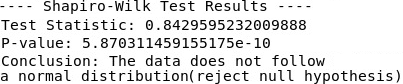
\includegraphics[width=1\linewidth]{img/mandelbrot_shapiro_test_energy_update.png}
    \caption{Shapiro-Wilk test results for Energy(\texttt{mandelbrot} program)}
    \label{fig:Shapiro-Wilk test results for Energy for mandelbrot}
  \end{minipage}
  \hfill
  \begin{minipage}[b]{0.49\textwidth}
    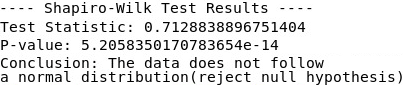
\includegraphics[width=1\linewidth]{img/mandelbrot_shapiro_test_power_update.png}
    \caption{Shapiro-Wilk test results for Power(\texttt{mandelbrot} program)}
    \label{fig:Shapiro-Wilk test results for Power for mandelbrot}
  \end{minipage}
\end{figure}
\vspace{-8pt}

Moreover, Figures \ref{fig:Graph of total energy consumption for mandelbrot} and \ref{fig:Graph of total power consumption for mandelbrot} 
%provide insights into the overall usage patterns. 
shows the box-plot for the data distribution of energy and power consumption of the processes
%IDs (PIDs) 
related to the execution of the java program.
%in Figure \ref{fig:Boxplot of total energy consumption for mandelbrot} enhances our understanding by highlighting potential outliers and data distribution. 
These visual aids collectively facilitate a comprehensive interpretation of the energy and power behaviors observed.
For instance, 
%a clear pattern emerges, 
we can observe four distinct clusters for energy consumption. It corresponds to the script parameter values, we used 15 000, 20 000, 30 000, and 40 000 as parameters of the \texttt{mandelbrot} code. A greater value for the parameter, a higher energy consumption values. Because at least the time is extended. Seeing the graph related to power consumption there is a more stable use of CPU for executing the \texttt{mandelbrot} code. These clusters were formed over 30 iterations. %highlighting the consistent energy and power usage patterns. 
%Interestingly, the energy and power consumption graphs show proportional clusters, indicating a direct relationship between the two metrics.

%In Figures \ref{fig:Graph of total energy consumption for mandelbrot} and \ref{fig:Graph of total power consumption for mandelbrot}, the energy and power consumption of Java processes are mapped against their unique Process IDs (PIDs) respectively. A clear pattern emerges, revealing four distinct clusters that correspond to script parameter values of 15,000, 20,000, 30,000, and 40,000. These clusters are formed over 30 iterations, highlighting the consistent energy and power usage patterns. Interestingly, the energy and power consumption graphs show proportional clusters, indicating a direct relationship between the two metrics.

\vspace{-12pt} % Reduce space above figure
\setlength{\belowcaptionskip}{-13pt} % Reduce space below caption
\begin{figure}[htbp]
  \centering
  \begin{center}
    \begin{minipage}[b]{0.49\textwidth}
      \centering
      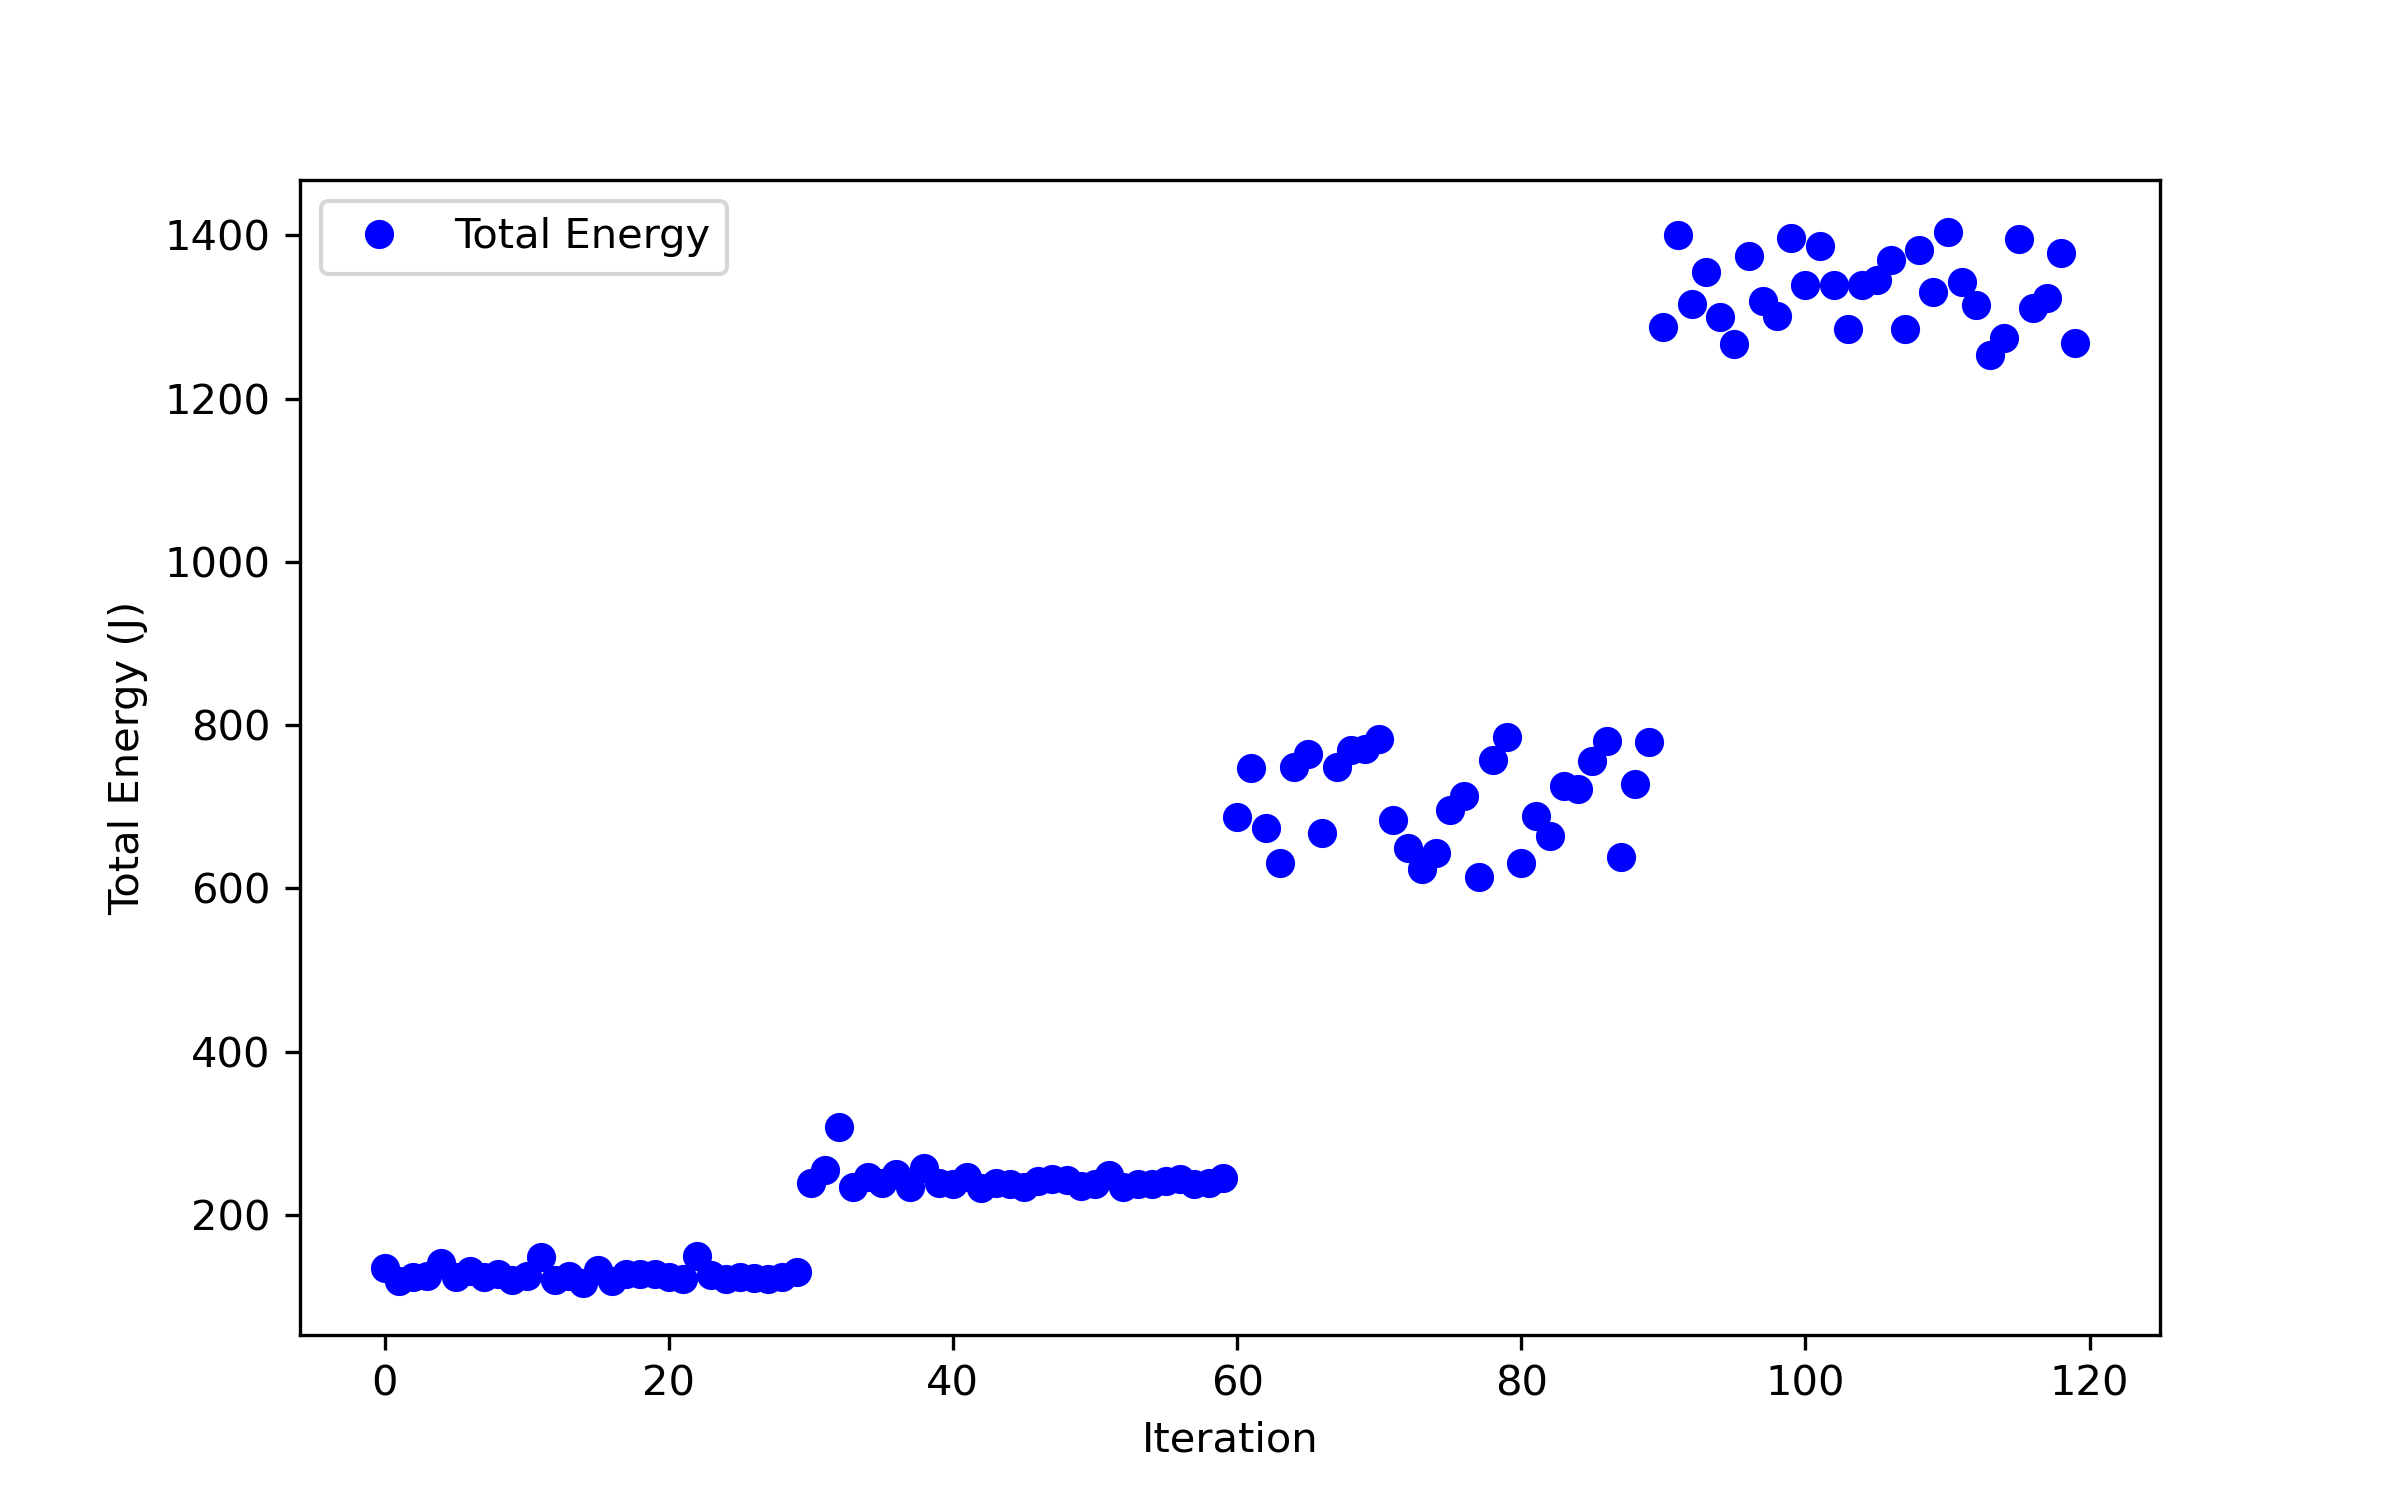
\includegraphics[width=\linewidth]{img/jx_total_energy_mandelbrot.png}
      \caption{Graph of total energy consumption(\texttt{mandelbrot} program)}
      \label{fig:Graph of total energy consumption for mandelbrot}
    \end{minipage}
    \hfill
    \begin{minipage}[b]{0.49\textwidth}
      \centering
      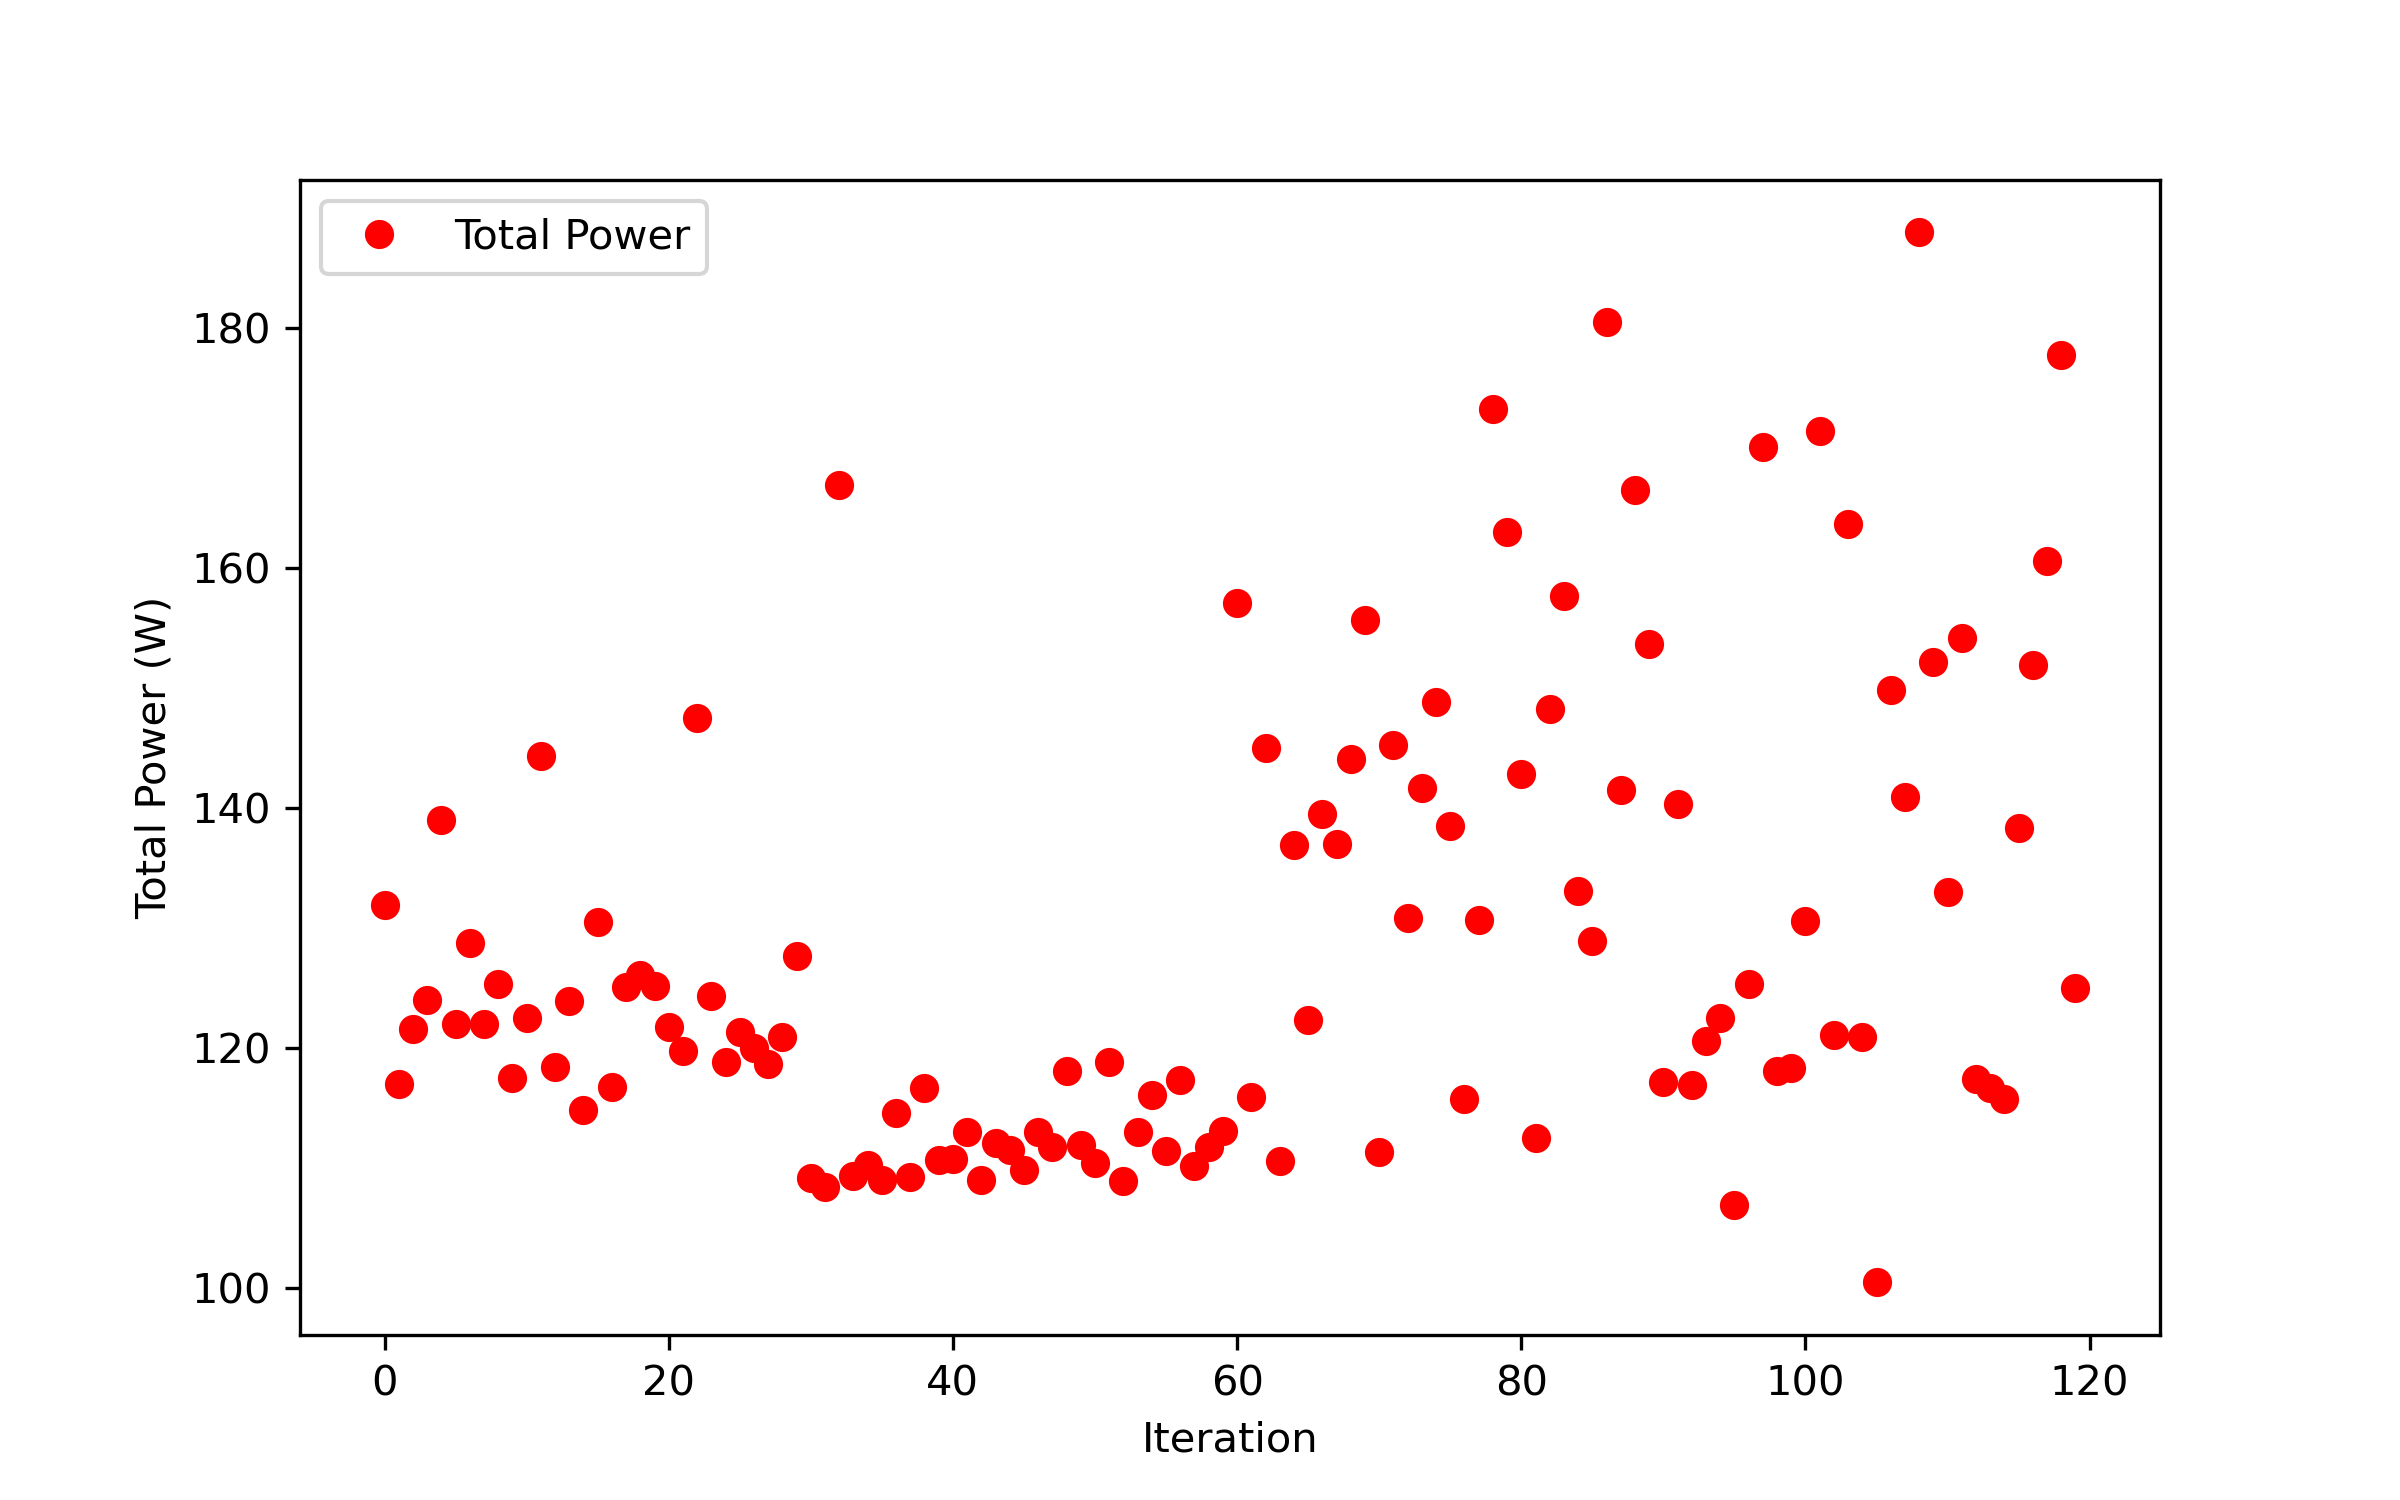
\includegraphics[width=\linewidth]{img/jx_total_power_mandelbrot.png}
      \caption{Graph of total power consumption(\texttt{mandelbrot} program)}
      \label{fig:Graph of total power consumption for mandelbrot}
    \end{minipage}
  \end{center}
\end{figure}
\vspace{-12pt} % Reduce space below figure


%\subsection{Energy consumption monitoring of a full project (cMath\_original) using JoularJX:} 
\vspace{-10pt}
\section{Energy consumption monitoring of a Java project} 

%In the second experiment, energy consumption for 'cMath\_original' was monitored using JoularJX 2.0. A test class, 'RunAllSuite.java', was executed using the \href{http://www.java2s.com/Code/Jar/c/Downloadcpsuite126jar.htm}{cpsuite-1.2.6.jar.zip} file and a script, 'jx\_script\_math.sh'. This script, containing various Python scripts, executed 'RunAllSuite.java' 30 times, managing resultant files in organized directories like "jx\_results". The Python scripts facilitated data extraction, processing, and graph generation from CSV files.The "shapiro\_wilk\_test\_energy.py" and "shapiro\_wilk\_test\_power.py" scripts assessed the normality of the energy and power data. The experiment was carried out by first cloning the repository from \url{https://gitlabev.imtbs-tsp.eu/sticamsud/enact-internship-2023.git} and navigating to the 'cMath\_original' directory within 'Prem\_Experiment'. After installation of JoularJX, as guided by its official website (\url{https://github.com/joular/joularjx}), the 'RunAllSuite.java' file located in 'src/test/java' was compiled. The resultant 'RunAllSuite.class' file was then moved to the 'bin' directory. The final step involved executing the 'jx\_script\_math.sh' script.


In the second experiment, the energy consumption of a Java project, \ie \texttt{cMath}\footnote{\texttt{cMath} was taken from the bench-marking used in~\cite{DBLP:conf/esem/SahinPC14} \url{https://bitbucket.org/udse/refactoring-study/src/master/} }, was monitored using \textit{JoularJX 2.0} as the previous experiment. 

\vspace{.5em}
%Similar to the previous experiment, \textit{JoularJX} was used to monitor energy and power consumption. %obtain updated tree structure results in the output directory. 
For a Java application, we execute its test cases classes that exercise the functionality of the Java application. The \texttt{cMath} application already contains a set of test cases classes. To execute all test cases of the project together, a new test class named \texttt{RunAllSuite.java} (see Appendix~\ref{sec:alltests} for more details) was created in the \texttt{test} directory. To execute the \texttt{RunAllSuite} class with JoularJX, it was necessary to download the \texttt{cpsuite-1.2.6}\footnote{\url{http://www.java2s.com/Code/Jar/c/Downloadcpsuite126jar.htm}} jar. 

\vspace{.5em}
A script called \texttt{jx\_script\_math.sh} in the \texttt{cMath} directory was created and used to execute the \texttt{RunAllSuite} class, which captured power and energy measurements using the JoularJX and managed the resulting files. 

%The script included several Python files: "jx\_gatherData.py," "jx\_plot.py," "jx\_process\_level\_methods.py," "shapiro\_wilk\_test\_energy.py," and "shapiro\_wilk\_test\_power.py." 

%The script set up directories for storing output files. These directories included "jx\_results" as the main folder, which contained subfolders for "energy", "energy\_filtered", "power", and "power\_filtered". Each of these subfolders further contained "methods" and "calltrees" directories.

\vspace{.5em}
The script sets the Java classpath for using the \textit{JUnit} and the \texttt{cpsuite-1.2.6} jars,  and performs the \texttt{RunAllSuite} java program in a loop for 30 iterations.
%
And, the script is based on the \texttt{jx\_script.sh} script (see Appendix~\ref{sec:mainscript}). So, the steps that it executes are the same than the previous experiment.

%During the first iteration, the output was saved to a file named 'java\_temp.pmb,' and for subsequent iterations, the output was discarded. After each execution, four types of files were created by JoularJX, representing energy and power data at different levels of granularity. These files had specific names based on the process ID of the Java program. The script then moved the non-empty files to their respective directories under "jx\_results". If a file was empty, it was deleted.

%Once the iterations were completed, the script proceeded to execute Python scripts for further data processing and analysis. The script "jx\_gatherData.py" read energy and power data from CSV files in specific directories and created Pandas data frames to store the data. The data frames were then processed to extract relevant information (such as method names, parameters, iterations, and energy/power consumption), and this information was stored in lists. The lists were then used to create new data frames with meaningful column names, which were then saved to CSV files. After that, the "jx\_process\_level\_methods.py" script read data from a CSV file containing energy and power consumption values for different iterations of a process. It then calculated the total and average energy consumption, and total and average power consumption for each process id, and wrote these results to a new CSV file. The code used the Python CSV module to read and write CSV files and stored the results in dictionaries. The "jx\_process\_level\_methods.py" script analyzed the power consumption data at the method level, calculating energy and power for each method. The "jx\_plot.py" script generated graphs based on the gathered data. Subsequently, the "jx\_plot\_geom\_boxplot.py" script created box plots to visualize the total energy consumption across all process IDs.

%Lastly, the script ran the "shapiro\_wilk\_test\_energy.py" and "shapiro\_wilk\_test\_power.py" scripts, which performed Shapiro\-Wilk tests to check for normality in the energy and power consumption data, respectively.\par

\subsection{Experimental Results and Analysis} 

In this section, we analyze the energy and power consumption data of the \textit{cMath} project. Figures \ref{fig:Shapiro-Wilk test results for Energy for cMath project} and \ref{fig:Shapiro-Wilk test results for Power for cMath project} depict the Shapiro-Wilk test results for energy and power data distributions. 
%These figures shed light on the distribution patterns of the data. 
%
%The Shapiro-Wilk test was performed on the data for "energy" and "power" from the cMath\_Original project to evaluate their normality. 
The test statistics obtained were $0.907$ and $0.864$ with \textit{p-values} of $0.013$ and $0.001$, respectively. Given these \textit{p-values} are below the $0.05$ significance level, we can reject the null hypothesis and conclude that the data for both measurements, \ie energy and power consumption, is not normally distributed.
%corroborated by visual assessments of their respective plots (figures \ref{fig:Shapiro-Wilk test results for Energy for cMath project} and \ref{fig:Shapiro-Wilk test results for Power for cMath project}).

\begin{figure}[h!]
  \centering
  \begin{minipage}[b]{0.49\textwidth}
    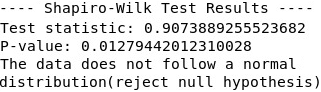
\includegraphics[width=.8\linewidth]{img/cMath_project_shapiro_test_energy_update.png}
    \caption{Shapiro-Wilk test results for Energy(\texttt{cMath} project)}
    \label{fig:Shapiro-Wilk test results for Energy for cMath project}
  \end{minipage}
  \hfill
  \begin{minipage}[b]{0.49\textwidth}
    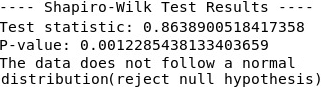
\includegraphics[width=.8\linewidth]{img/cMath_project_shapiro_test_power_update.png}
    \caption{Shapiro-Wilk test results for Power(\texttt{cMath} project)}
    \label{fig:Shapiro-Wilk test results for Power for cMath project}
  \end{minipage}
\end{figure}

%We also visually assess the overall consumption patterns using the graphs for total energy (Figure \ref{fig:Graph of total energy consumption for cMath project}) and power (Figure \ref{fig:Graph of total power consumption for cMath project}). A Boxplot analysis on the total energy consumption is presented in Figure \ref{fig:Boxplot of total energy consumption for cMath project} to highlight distribution and possible outliers.
\vspace{.5em}
Moreover, Figures \ref{fig:Graph of total energy consumption for cMath project} and \ref{fig:Graph of total power consumption for cMath project} shows the box-plot for the data distribution of energy and power consumption 
%represent energy and power consumption patterns against 
of process IDs (PID) from the execution of the Java application. The energy consumption varies between 1200 and 1320 joules with an average range of 1240 to 1320 joules, showing a noticeable spike between PIDs 54000 and 54500. Meanwhile, power consumption ranges from 10 to 80 Watts, averaging between 5 and 40 wards, with two notable peaks near 80 wards between PIDs 53500 and 54000. 
%These patterns help identify methods with high energy and power demands, which could benefit from optimization.

\begin{figure}[htbp]
  \centering
  \begin{center}
    \begin{minipage}[b]{0.49\textwidth}
      \centering
      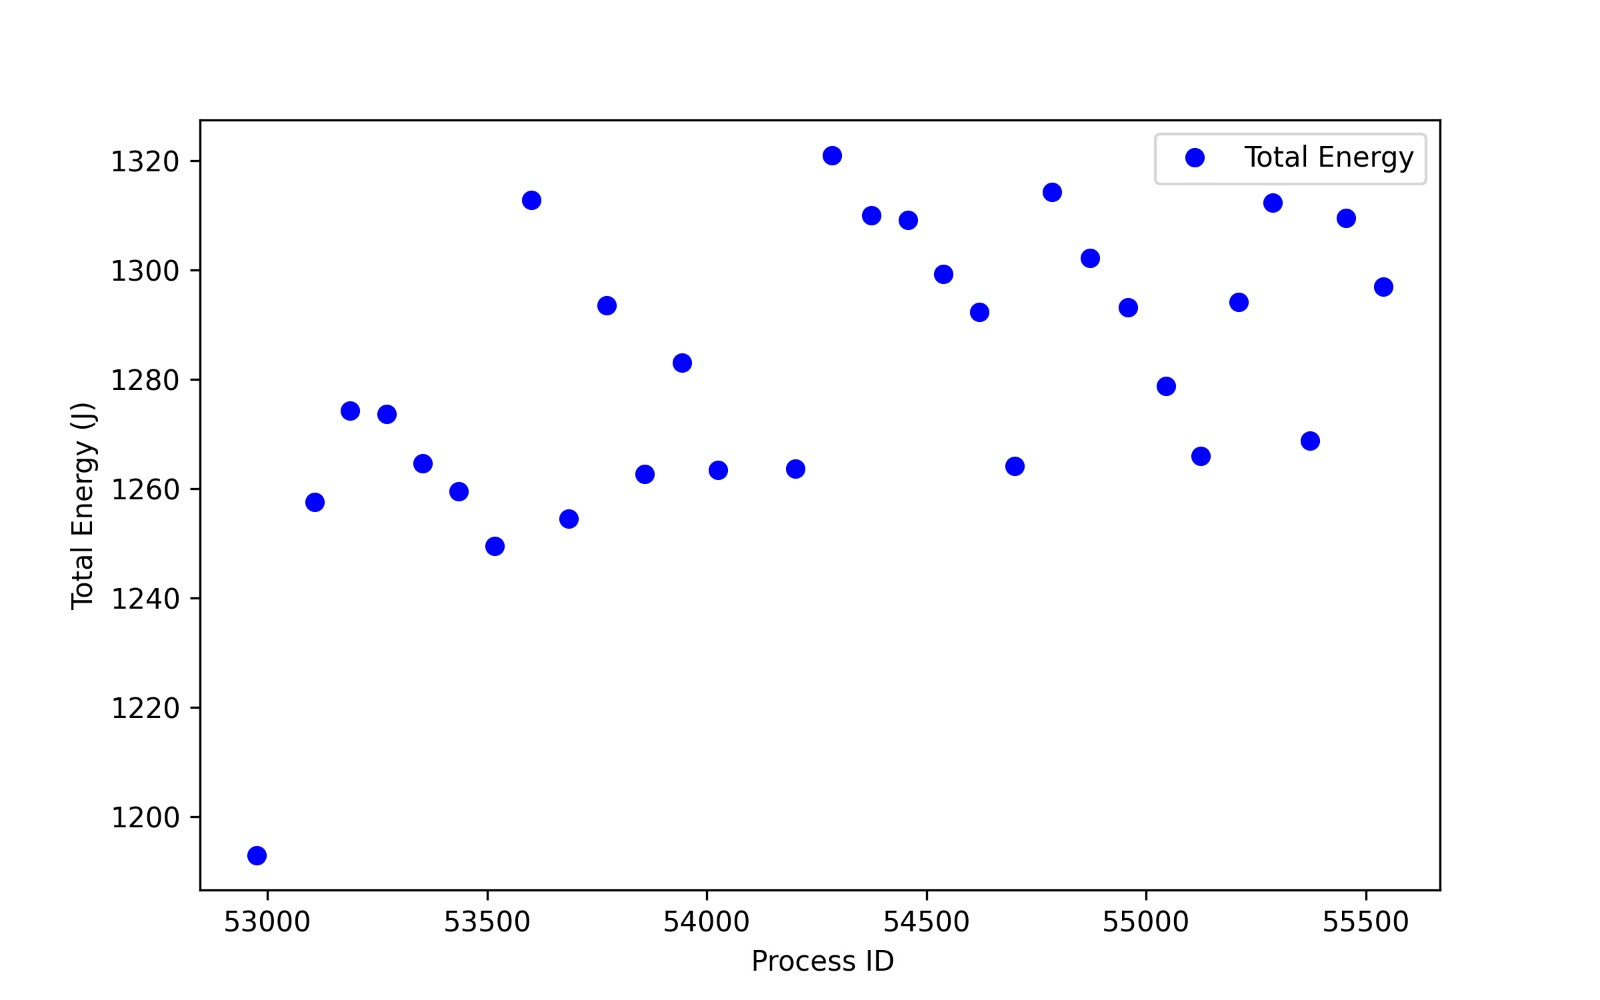
\includegraphics[width=\linewidth]{img/cMath_project_energy.jpeg}
      \caption{Graph of total energy consumption(\texttt{cMath} project)}
      \label{fig:Graph of total energy consumption for cMath project}
    \end{minipage}
    \hfill
    \begin{minipage}[b]{0.49\textwidth}
      \centering
      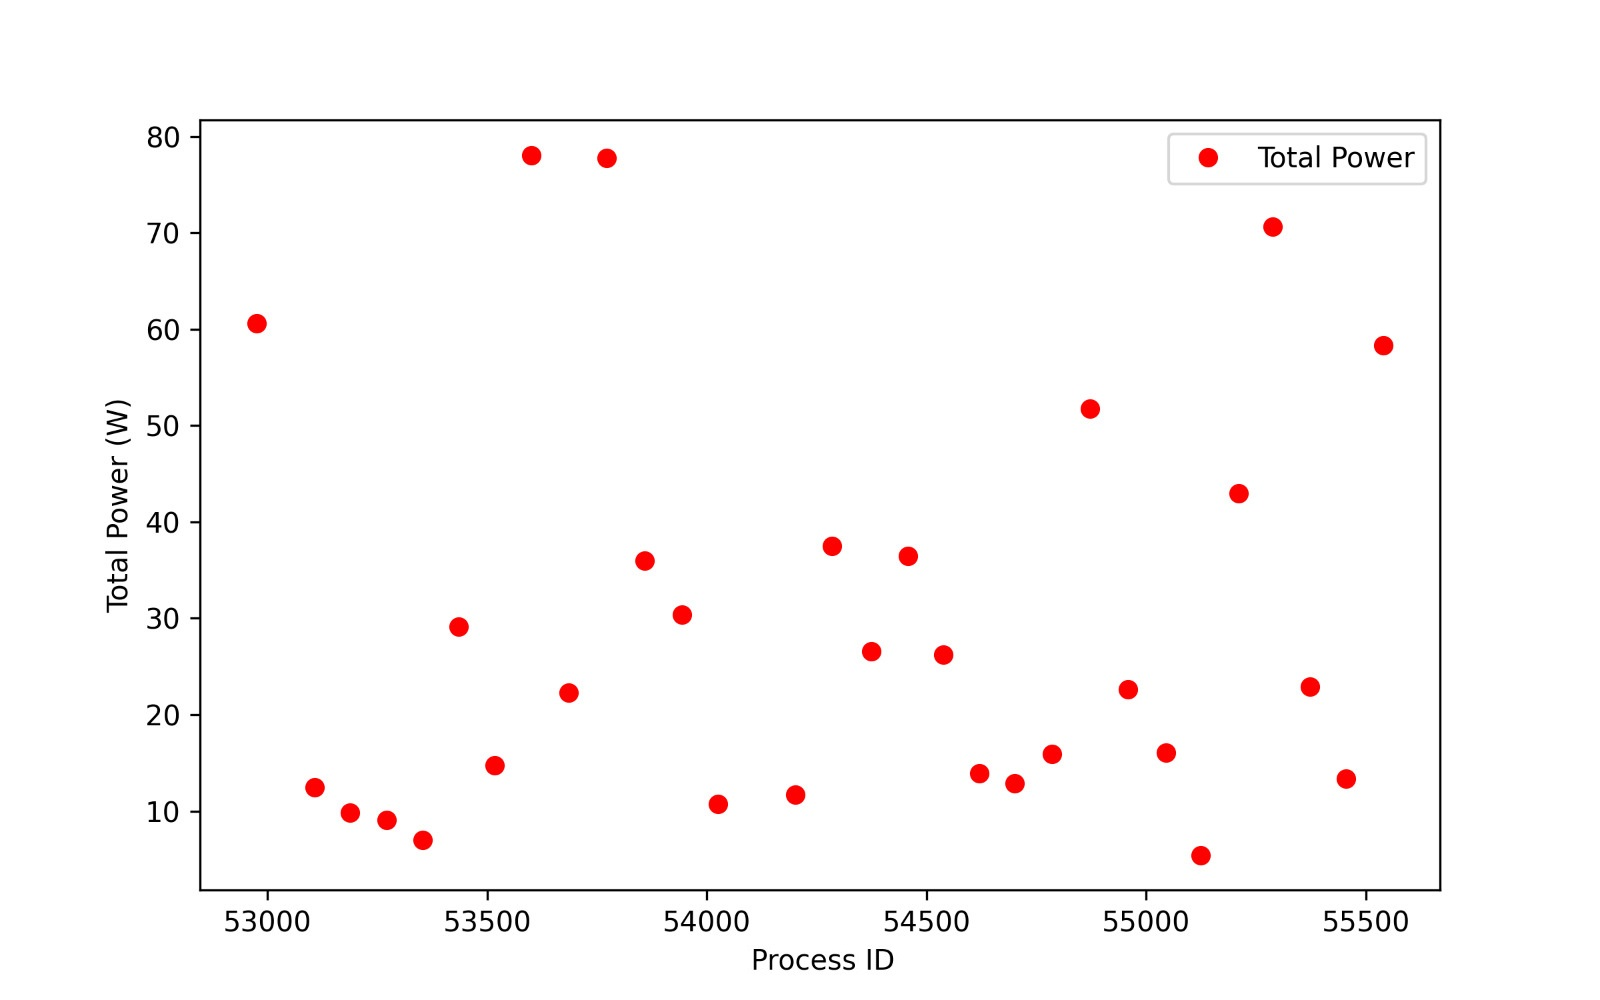
\includegraphics[width=\linewidth]{img/cMath_project_power.jpeg}
      \caption{Graph of total power consumption(\texttt{cMath} project)}
      \label{fig:Graph of total power consumption for cMath project}
    \end{minipage}
  \end{center}
\end{figure}

\vspace{10em}
In the analysis of the energy consumption for the \textit{cMath} project, as depicted in box-plot figure \ref{fig:Boxplot of total energy consumption for cMath project}, the proximity of the mean and median lines suggests a symmetric distribution, though the mean is slightly higher, hinting at some high consumption values. %Additionally, outliers on both sides of the whisker lines indicate unusual energy consumption values. 
This box-plot provides a comprehensive view of the project's typical energy usage, essential for its effective management.
\vspace{-10pt}
\begin{figure}[htbp]
  \centering
  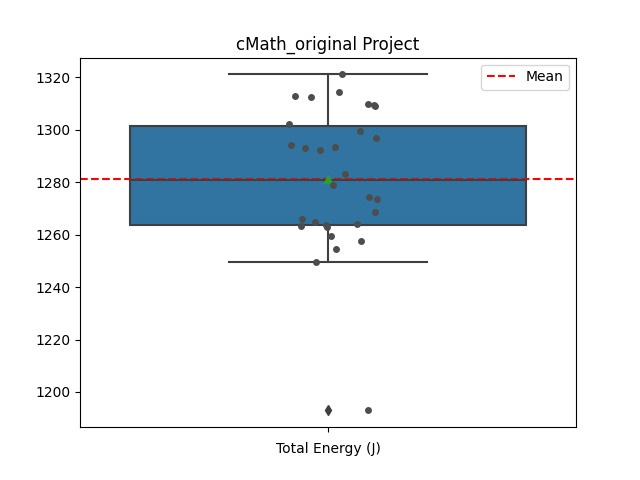
\includegraphics[width=.49\textwidth]{img/cMath_project_energy_boxplot.jpeg}
  \caption{Box-plot of total energy consumption(\texttt{cMath} project)}
  \label{fig:Boxplot of total energy consumption for cMath project}
\end{figure}
\vspace{-10pt}